\section{Sistema di identificazione}
Il meccanismo di identificazione è la procedura per verificare che un determinato dispositivo
è abilitato a connettersi alla rete.
Questo procedimento avviene tramite l'\textit{Authentication and key agreement} (AKA), procedimento in cui
il \textit{core network} abilita un dispositivo a connettersi.\\
Di seguito verranno illustrate le procedure di inteficazione per le principali generazioni cellulari: dal 2G al 5G. Il 
1G è stato escluso poiché ha un funzionamento completamente analogico.

\subsection{2G}
Nei sisteni di seconda generazione nella fase di autenticazione di un dispositivo vengono interpellati principalmente tre componenti:
\begin{enumerate}
    \item Il dispositivo cellulare con l'apposita SIM
    \item Il MSC di riferimento
    \item La HLR con l'AUC per effettuare la validazione
\end{enumerate}
\begin{figure}[ht]
    \centering
    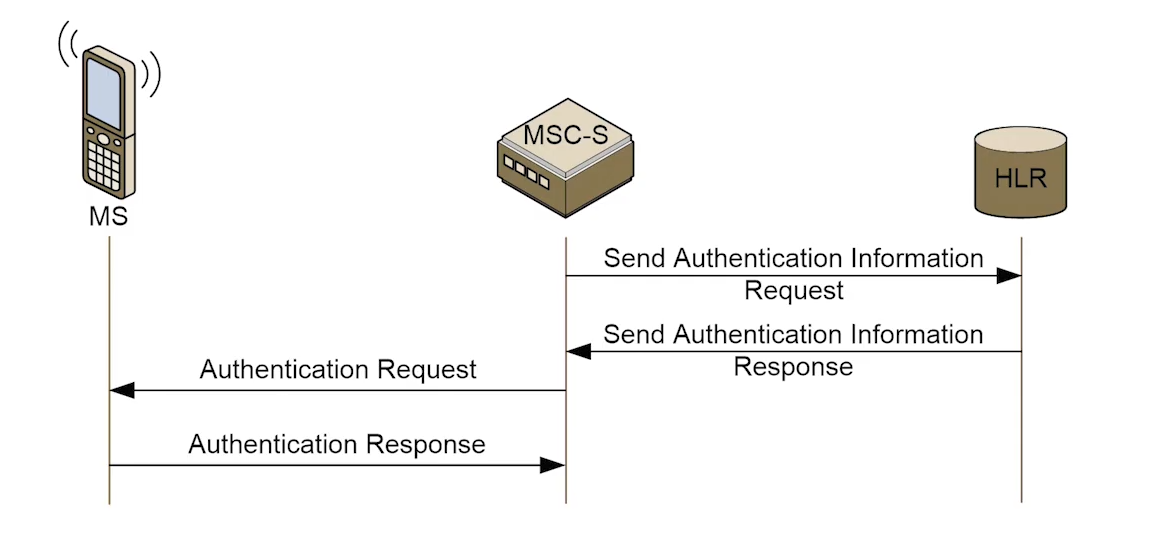
\includegraphics[width=0.7\textwidth]{images/identification-2g.png}
    \caption{Identificazione nelle reti 2G}
\end{figure}
Per autenticare un dispositivo vengono generati i vettori di autenticazione nell'AUC, univochi rispetto a un determinato dispositivo identificato da 
un IMSI. Questi vettori poi vengono inviati all'HLR che si occuperà do verificarne la correttezza e inviare una risposta al MSC che la inoltra al MS.

\subsection{3G}
Nei sistemi di terza generazione i componenti utilizzati per l'identificazione di un dispositivo sono gli stessi della generazione precedente salvo qualche 
eccezione. Come illustrato precedentemente, come nel GPRS nelle reti 3G ci sono due \textit{Switcing centre}: MSC per il classico circuito telefonico e il GMSC per 
i pacchetti di rete. L'identificazione viene completata allo stesso modo della seconda generazione, ma 

Con rete 3G si intendono l'insieme delle tecnologie di terza generazione, stiamo quindi parlando di un'architettura UMTS.
Un \acrshort{ms} che si vuole collegare alla rete deve procedere con la fase di autenticazione o identificazione anche detta \textit{Authentication and key agreement}
(AKA). In questa fase, viene interrogata la rispettiva HLR/AuC dove l'IMSI del dispositivo viene validato, se tutto procede correttamente
viene notificato il SGSN che inoltra al \acrshort{ms} l'avviso di autenticazione completata.
%Schema autenticazione umts

\subsection{4G}

\subsection{5G}